%---------------------------------------------------------------
        %% SOM
        %-----------------------------------------
        %% linkes Bild
        \begin{tikzpicture}[>=stealth', node distance=\layersep cm, shorten >=1pt]
        \def\layersep{2}            % vertikal distance between the layers
        \def\neuronsep{1.5}         % Horizontal distance between neurons
        \def\dlsize{1.5}            % distance between node and layer lable
        \def\inout{\layersep*.65}   % Size of in- and output-arrow
        \def\siz{.8}                % neuronsize
        \def\y{3}                   % Start of the most upper layer
        \def\ni{5}                  % Amount of input neurons
        \def\no{3}                  % Amount of output neurons
        \tikzstyle{neuron}=[circle,draw=black,minimum size=\siz cm,inner sep=2pt]
        \tikzstyle{annot} = [text width=6em, text centered]
        \tikzset{fontscale/.style = {font={\fontsize{#1pt}{#1pt}\selectfont}}}
        \tikzset{
                ident/.pic={
                \draw[semithick] (-\siz/#1,-\siz/#1) -- (\siz/#1,\siz/#1);
            }}
        \newcommand{\neurono}[3][]{%
        \ifthenelse{\equal{#3}{0}}{%
            \node[neuron,circle split,inner sep=1pt,fontscale=6] (#1) at (#2) { $\mathbf{||c,x||}$ \nodepart{lower}};
            \node[fontscale=6] at ($(#2.lower)-(0,\siz/4)$){\textbf{Gauß}};
            }{
            \node[neuron,circle split,inner sep=1.3pt] (#1) at (#2)
                    {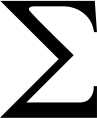
\includegraphics[width=0.225cm]{Bilder/Sigma.png} \nodepart{lower} };
            \pic at ($(#1.lower)-(0,\siz/8)$) {ident=#3};
            }}
        % Draw the left input layer nodes
            \foreach \xn in {1,...,\ni}{
                \node[neuron,fontscale=15] (Il-\xn) at (\xn*\neuronsep-\neuronsep,\y) {$i_{\xn}$};
                \node[above of=Il-\xn, node distance=\inout cm] (Inl-\xn) {};
                \draw [arrows={-Stealth[length=7pt]},densely dotted] (Inl-\xn) edge (Il-\xn);
            }
        % Draw the output layer node
            \foreach \xn in {1,...,\no}{
                \node[neuron] (Ol-\xn) at ({(\ni-1)*\neuronsep/2-\neuronsep/2*(\no-1)+(\xn-1)*\neuronsep},\y-\layersep) [fontscale=15] {$\Omega_{\xn}$};
        % Connect every node in the input layer with the output layer                
            \foreach \source in {1,...,\ni}{
                \draw [->,arrows={-Stealth[length=7pt]}] (Il-\source) edge (Ol-\xn);}}
        % Connect every node in the output layer
            \pgfmathsetmacro{\nom}{\no - 1}
            \ifthenelse{\equal{\no}{1}}{%
            }{
               \foreach \xn in {1,...,\nom}{
                    \pgfmathtruncatemacro{\xnp}{\xn + 1}
                    \draw[arrows={Stealth[length=7pt]-Stealth[length=7pt]},shorten <=1pt] (Ol-\xn) edge[bend right=45] (Ol-\xnp);
            }}
        % Annotate the layers
                \node[annot,right of=Il-\ni, node distance=\dlsize cm] (il) {\textbf{Eingabe- schicht}};
                \node[annot,below of=il] {\textbf{Ausgabe- schicht}};
        %-----------------------------------------
        %% rechtes Bild
        % Draw the right input layer nodes
                \coordinate (tIr) at ($(il)-(Il-\ni)$);
                \coordinate (ttIr) at (tIr |- 0,0);
                \coordinate (Ir) at ($(il)+(ttIr)$);
            \foreach \name / \xn in {1,...,\ni}{
        % This is the same as writing \foreach \name / \y in {1/1,2/2,3/3,4/4}
                \node[neuron] (Ir-\xn) at ($(Ir)+(\xn*\neuronsep-\neuronsep,0)$) {};
                \node[above of=Ir-\xn, node distance=\inout cm] (Inr-\xn) {};
                \pic at (Ir-\xn) {ident=4};
                \draw [->,arrows={-Stealth[length=7pt]},densely dotted] (Inr-\xn) edge (Ir-\xn);}
        % Draw the right output layer node
            \foreach \xn in {1,...,\no}{
                \neurono[Or-\xn]{$(Ir)+({(\ni-1)*\neuronsep/2-\neuronsep/2*(\no-1)+(\xn-1)*\neuronsep},-\layersep)$}{0}
                \node[node distance=\inout cm, below of=Or-\xn] (Onr) {};
                %\draw [->,arrows={-Stealth[length=7pt]},densely dotted] (Or-\xn) edge (Onr);
        % Connect every node in the hidden layer with the output layer
            \foreach \source in {1,...,\ni}
                \draw [arrows={-Stealth[length=7pt]}] (Ir-\source) edge  (Or-\xn);
            }
                \node[fill=white,inner sep=1pt,fontscale=10] at ($(Or-1)+({(\no-1)*\neuronsep/2},\layersep*.55)$) {$\dots\, w_{i,\Omega}\,\dots$};
        % Connect every node in the output layer
            \ifthenelse{\equal{\no}{1}}{%
            }{
               \foreach \xn in {1,...,\nom}{
                    \pgfmathtruncatemacro{\xnp}{\xn + 1}
                    \draw[arrows={Stealth[length=7pt]-Stealth[length=7pt]},shorten <=1pt] (Or-\xn) edge[bend right=45] (Or-\xnp);
            }}
        \end{tikzpicture}